\documentclass[aspectratio=169]{beamer}
% Shared preamble for ml/ slide decks.
% Each lecture .tex starts with:
%   \documentclass[aspectratio=169]{beamer}
%   % Shared preamble for ml/ slide decks.
% Each lecture .tex starts with:
%   \documentclass[aspectratio=169]{beamer}
%   % Shared preamble for ml/ slide decks.
% Each lecture .tex starts with:
%   \documentclass[aspectratio=169]{beamer}
%   \input{../preamble}
% Compile from inside the chapter folder so \input{../preamble} resolves.

\usetheme{default}
\usecolortheme{dove}

\setbeamertemplate{navigation symbols}{}
\setbeamertemplate{footline}{%
  \hfill{\large\insertframenumber\,/\,\inserttotalframenumber}\hspace{0.8em}\vspace{0.5em}%
}

% Project palette (existing, kept for backwards compatibility with deferred/*)
\definecolor{popblue}{RGB}{52, 101, 164}
\definecolor{sampred}{RGB}{204, 0, 0}
\definecolor{paramgreen}{RGB}{0, 140, 70}
\definecolor{warnred}{RGB}{180, 40, 40}
\definecolor{orange1}{RGB}{220, 120, 0}
\definecolor{violet1}{RGB}{120, 50, 160}
\definecolor{lightbg}{RGB}{245, 245, 250}

% Armenian flag palette (use these for any 3-color highlight; per CLAUDE.md).
% "Nice versions": slightly de-saturated from the official spec for slide use,
% so they don't burn out under projector colors. Originals kept as *_pure.
\definecolor{armred}{RGB}{200, 30, 40}      % nice red (official #D90012 muted)
\definecolor{armblue}{RGB}{30, 70, 160}     % nice blue (official #0033A0 muted)
\definecolor{armorange}{RGB}{230, 160, 30}  % nice orange (official #F2A800 muted)
\definecolor{armred_pure}{HTML}{D90012}     % official Armenian flag red
\definecolor{armblue_pure}{HTML}{0033A0}    % official Armenian flag blue
\definecolor{armorange_pure}{HTML}{F2A800}  % official Armenian flag orange

\setbeamercolor{frametitle}{fg=popblue}
\setbeamercolor{title}{fg=popblue}

\usepackage{pgfplots}
\usepackage{tikz}
\usetikzlibrary{shapes, arrows.meta, positioning, calc, decorations.pathreplacing, patterns, matrix}
\pgfplotsset{compat=1.18}
\usepackage{amsmath, amssymb, amsfonts}
\usepackage{bm}
\usepackage{dsfont}
\usepackage{array}
\usepackage{pifont}
\usepackage{colortbl}
\usepackage{fontenc}

% Callout boxes. Purely additive - existing decks are unaffected.
% Usage: \begin{tcolorbox}[colback=armblue!8, colframe=armblue, boxrule=0.6pt, arc=2pt,
%                          title=\textbf{Key idea}] ... \end{tcolorbox}
% Palette convention (ml/SLIDE_STYLE.md): armblue=key idea, armred=trap/warning,
% paramgreen=takeaway or "Next", armorange=watch-out.
\usepackage[most]{tcolorbox}

% Cleaner table rules (\toprule, \midrule, \bottomrule). Also purely additive.
\usepackage{booktabs}

% \cancel{...} for struck-through terms in derivations (added 2026-08-11 for the
% importance-sampling frame in ch11_rl, where the dynamics cancel). Purely additive.
\usepackage{cancel}

% Minimal ML notation macros (subset of slds-lmu latex-math/basic-ml.tex).
% Kept here so we don't have to inline-expand every \thetav, \xv, etc.
% when porting upstream slides.
\newcommand{\R}{\mathds{R}}
\newcommand{\N}{\mathds{N}}
\newcommand{\E}{\mathds{E}}
\newcommand{\Xspace}{\mathcal{X}}
\newcommand{\Yspace}{\mathcal{Y}}
\newcommand{\Hspace}{\mathcal{H}}
\newcommand{\D}{\mathcal{D}}
\newcommand{\Dtrain}{\mathcal{D}_{\text{train}}}
\newcommand{\Dtest}{\mathcal{D}_{\text{test}}}
\newcommand{\xv}{\mathbf{x}}
\newcommand{\yv}{\mathbf{y}}
\newcommand{\Xmat}{\mathbf{X}}
\newcommand{\id}{\mathbf{I}}
\newcommand{\thetav}{\bm{\theta}}
\newcommand{\thetah}{\hat{\bm{\theta}}}
\newcommand{\lamv}{\bm{\lambda}}
\newcommand{\fx}{f(\xv)}
\newcommand{\fxt}{f(\xv \,|\, \bm{\theta})}
\newcommand{\fxi}{f\!\left(\xv^{(i)}\right)}
\newcommand{\fh}{\hat{f}}
\newcommand{\fxh}{\hat{f}(\xv)}
\newcommand{\yh}{\hat{y}}
\newcommand{\yih}{\hat{y}^{(i)}}
% \xi clashes with the Greek letter \xi; write \xv^{(i)} inline instead.
\newcommand{\yi}[1][i]{y^{(#1)}}
\newcommand{\xyi}[1][i]{\left(\xv^{(#1)},\, y^{(#1)}\right)}
\newcommand{\thx}{\bm{\theta}^\top \xv}
\newcommand{\sumin}{\sum_{i=1}^{n}}
\newcommand{\sumjp}{\sum_{j=1}^{p}}
\newcommand{\Lxy}{L\!\left(y, \fx\right)}
\newcommand{\Lxyi}{L\!\left(\yi, \fxi\right)}
\newcommand{\risk}{\mathcal{R}}
\newcommand{\riske}{\mathcal{R}_{\text{emp}}}
\newcommand{\risket}{\mathcal{R}_{\text{emp}}(\bm{\theta})}
\newcommand{\riskt}{\mathcal{R}(\bm{\theta})}
\newcommand{\riskr}{\mathcal{R}_{\text{reg}}}
\newcommand{\argmin}{\mathop{\mathrm{arg\,min}}}
\newcommand{\argmax}{\mathop{\mathrm{arg\,max}}}
\newcommand{\eps}{\varepsilon}

% Compile from inside the chapter folder so % Shared preamble for ml/ slide decks.
% Each lecture .tex starts with:
%   \documentclass[aspectratio=169]{beamer}
%   \input{../preamble}
% Compile from inside the chapter folder so \input{../preamble} resolves.

\usetheme{default}
\usecolortheme{dove}

\setbeamertemplate{navigation symbols}{}
\setbeamertemplate{footline}{%
  \hfill{\large\insertframenumber\,/\,\inserttotalframenumber}\hspace{0.8em}\vspace{0.5em}%
}

% Project palette (existing, kept for backwards compatibility with deferred/*)
\definecolor{popblue}{RGB}{52, 101, 164}
\definecolor{sampred}{RGB}{204, 0, 0}
\definecolor{paramgreen}{RGB}{0, 140, 70}
\definecolor{warnred}{RGB}{180, 40, 40}
\definecolor{orange1}{RGB}{220, 120, 0}
\definecolor{violet1}{RGB}{120, 50, 160}
\definecolor{lightbg}{RGB}{245, 245, 250}

% Armenian flag palette (use these for any 3-color highlight; per CLAUDE.md).
% "Nice versions": slightly de-saturated from the official spec for slide use,
% so they don't burn out under projector colors. Originals kept as *_pure.
\definecolor{armred}{RGB}{200, 30, 40}      % nice red (official #D90012 muted)
\definecolor{armblue}{RGB}{30, 70, 160}     % nice blue (official #0033A0 muted)
\definecolor{armorange}{RGB}{230, 160, 30}  % nice orange (official #F2A800 muted)
\definecolor{armred_pure}{HTML}{D90012}     % official Armenian flag red
\definecolor{armblue_pure}{HTML}{0033A0}    % official Armenian flag blue
\definecolor{armorange_pure}{HTML}{F2A800}  % official Armenian flag orange

\setbeamercolor{frametitle}{fg=popblue}
\setbeamercolor{title}{fg=popblue}

\usepackage{pgfplots}
\usepackage{tikz}
\usetikzlibrary{shapes, arrows.meta, positioning, calc, decorations.pathreplacing, patterns, matrix}
\pgfplotsset{compat=1.18}
\usepackage{amsmath, amssymb, amsfonts}
\usepackage{bm}
\usepackage{dsfont}
\usepackage{array}
\usepackage{pifont}
\usepackage{colortbl}
\usepackage{fontenc}

% Callout boxes. Purely additive - existing decks are unaffected.
% Usage: \begin{tcolorbox}[colback=armblue!8, colframe=armblue, boxrule=0.6pt, arc=2pt,
%                          title=\textbf{Key idea}] ... \end{tcolorbox}
% Palette convention (ml/SLIDE_STYLE.md): armblue=key idea, armred=trap/warning,
% paramgreen=takeaway or "Next", armorange=watch-out.
\usepackage[most]{tcolorbox}

% Cleaner table rules (\toprule, \midrule, \bottomrule). Also purely additive.
\usepackage{booktabs}

% \cancel{...} for struck-through terms in derivations (added 2026-08-11 for the
% importance-sampling frame in ch11_rl, where the dynamics cancel). Purely additive.
\usepackage{cancel}

% Minimal ML notation macros (subset of slds-lmu latex-math/basic-ml.tex).
% Kept here so we don't have to inline-expand every \thetav, \xv, etc.
% when porting upstream slides.
\newcommand{\R}{\mathds{R}}
\newcommand{\N}{\mathds{N}}
\newcommand{\E}{\mathds{E}}
\newcommand{\Xspace}{\mathcal{X}}
\newcommand{\Yspace}{\mathcal{Y}}
\newcommand{\Hspace}{\mathcal{H}}
\newcommand{\D}{\mathcal{D}}
\newcommand{\Dtrain}{\mathcal{D}_{\text{train}}}
\newcommand{\Dtest}{\mathcal{D}_{\text{test}}}
\newcommand{\xv}{\mathbf{x}}
\newcommand{\yv}{\mathbf{y}}
\newcommand{\Xmat}{\mathbf{X}}
\newcommand{\id}{\mathbf{I}}
\newcommand{\thetav}{\bm{\theta}}
\newcommand{\thetah}{\hat{\bm{\theta}}}
\newcommand{\lamv}{\bm{\lambda}}
\newcommand{\fx}{f(\xv)}
\newcommand{\fxt}{f(\xv \,|\, \bm{\theta})}
\newcommand{\fxi}{f\!\left(\xv^{(i)}\right)}
\newcommand{\fh}{\hat{f}}
\newcommand{\fxh}{\hat{f}(\xv)}
\newcommand{\yh}{\hat{y}}
\newcommand{\yih}{\hat{y}^{(i)}}
% \xi clashes with the Greek letter \xi; write \xv^{(i)} inline instead.
\newcommand{\yi}[1][i]{y^{(#1)}}
\newcommand{\xyi}[1][i]{\left(\xv^{(#1)},\, y^{(#1)}\right)}
\newcommand{\thx}{\bm{\theta}^\top \xv}
\newcommand{\sumin}{\sum_{i=1}^{n}}
\newcommand{\sumjp}{\sum_{j=1}^{p}}
\newcommand{\Lxy}{L\!\left(y, \fx\right)}
\newcommand{\Lxyi}{L\!\left(\yi, \fxi\right)}
\newcommand{\risk}{\mathcal{R}}
\newcommand{\riske}{\mathcal{R}_{\text{emp}}}
\newcommand{\risket}{\mathcal{R}_{\text{emp}}(\bm{\theta})}
\newcommand{\riskt}{\mathcal{R}(\bm{\theta})}
\newcommand{\riskr}{\mathcal{R}_{\text{reg}}}
\newcommand{\argmin}{\mathop{\mathrm{arg\,min}}}
\newcommand{\argmax}{\mathop{\mathrm{arg\,max}}}
\newcommand{\eps}{\varepsilon}
 resolves.

\usetheme{default}
\usecolortheme{dove}

\setbeamertemplate{navigation symbols}{}
\setbeamertemplate{footline}{%
  \hfill{\large\insertframenumber\,/\,\inserttotalframenumber}\hspace{0.8em}\vspace{0.5em}%
}

% Project palette (existing, kept for backwards compatibility with deferred/*)
\definecolor{popblue}{RGB}{52, 101, 164}
\definecolor{sampred}{RGB}{204, 0, 0}
\definecolor{paramgreen}{RGB}{0, 140, 70}
\definecolor{warnred}{RGB}{180, 40, 40}
\definecolor{orange1}{RGB}{220, 120, 0}
\definecolor{violet1}{RGB}{120, 50, 160}
\definecolor{lightbg}{RGB}{245, 245, 250}

% Armenian flag palette (use these for any 3-color highlight; per CLAUDE.md).
% "Nice versions": slightly de-saturated from the official spec for slide use,
% so they don't burn out under projector colors. Originals kept as *_pure.
\definecolor{armred}{RGB}{200, 30, 40}      % nice red (official #D90012 muted)
\definecolor{armblue}{RGB}{30, 70, 160}     % nice blue (official #0033A0 muted)
\definecolor{armorange}{RGB}{230, 160, 30}  % nice orange (official #F2A800 muted)
\definecolor{armred_pure}{HTML}{D90012}     % official Armenian flag red
\definecolor{armblue_pure}{HTML}{0033A0}    % official Armenian flag blue
\definecolor{armorange_pure}{HTML}{F2A800}  % official Armenian flag orange

\setbeamercolor{frametitle}{fg=popblue}
\setbeamercolor{title}{fg=popblue}

\usepackage{pgfplots}
\usepackage{tikz}
\usetikzlibrary{shapes, arrows.meta, positioning, calc, decorations.pathreplacing, patterns, matrix}
\pgfplotsset{compat=1.18}
\usepackage{amsmath, amssymb, amsfonts}
\usepackage{bm}
\usepackage{dsfont}
\usepackage{array}
\usepackage{pifont}
\usepackage{colortbl}
\usepackage{fontenc}

% Callout boxes. Purely additive - existing decks are unaffected.
% Usage: \begin{tcolorbox}[colback=armblue!8, colframe=armblue, boxrule=0.6pt, arc=2pt,
%                          title=\textbf{Key idea}] ... \end{tcolorbox}
% Palette convention (ml/SLIDE_STYLE.md): armblue=key idea, armred=trap/warning,
% paramgreen=takeaway or "Next", armorange=watch-out.
\usepackage[most]{tcolorbox}

% Cleaner table rules (\toprule, \midrule, \bottomrule). Also purely additive.
\usepackage{booktabs}

% \cancel{...} for struck-through terms in derivations (added 2026-08-11 for the
% importance-sampling frame in ch11_rl, where the dynamics cancel). Purely additive.
\usepackage{cancel}

% Minimal ML notation macros (subset of slds-lmu latex-math/basic-ml.tex).
% Kept here so we don't have to inline-expand every \thetav, \xv, etc.
% when porting upstream slides.
\newcommand{\R}{\mathds{R}}
\newcommand{\N}{\mathds{N}}
\newcommand{\E}{\mathds{E}}
\newcommand{\Xspace}{\mathcal{X}}
\newcommand{\Yspace}{\mathcal{Y}}
\newcommand{\Hspace}{\mathcal{H}}
\newcommand{\D}{\mathcal{D}}
\newcommand{\Dtrain}{\mathcal{D}_{\text{train}}}
\newcommand{\Dtest}{\mathcal{D}_{\text{test}}}
\newcommand{\xv}{\mathbf{x}}
\newcommand{\yv}{\mathbf{y}}
\newcommand{\Xmat}{\mathbf{X}}
\newcommand{\id}{\mathbf{I}}
\newcommand{\thetav}{\bm{\theta}}
\newcommand{\thetah}{\hat{\bm{\theta}}}
\newcommand{\lamv}{\bm{\lambda}}
\newcommand{\fx}{f(\xv)}
\newcommand{\fxt}{f(\xv \,|\, \bm{\theta})}
\newcommand{\fxi}{f\!\left(\xv^{(i)}\right)}
\newcommand{\fh}{\hat{f}}
\newcommand{\fxh}{\hat{f}(\xv)}
\newcommand{\yh}{\hat{y}}
\newcommand{\yih}{\hat{y}^{(i)}}
% \xi clashes with the Greek letter \xi; write \xv^{(i)} inline instead.
\newcommand{\yi}[1][i]{y^{(#1)}}
\newcommand{\xyi}[1][i]{\left(\xv^{(#1)},\, y^{(#1)}\right)}
\newcommand{\thx}{\bm{\theta}^\top \xv}
\newcommand{\sumin}{\sum_{i=1}^{n}}
\newcommand{\sumjp}{\sum_{j=1}^{p}}
\newcommand{\Lxy}{L\!\left(y, \fx\right)}
\newcommand{\Lxyi}{L\!\left(\yi, \fxi\right)}
\newcommand{\risk}{\mathcal{R}}
\newcommand{\riske}{\mathcal{R}_{\text{emp}}}
\newcommand{\risket}{\mathcal{R}_{\text{emp}}(\bm{\theta})}
\newcommand{\riskt}{\mathcal{R}(\bm{\theta})}
\newcommand{\riskr}{\mathcal{R}_{\text{reg}}}
\newcommand{\argmin}{\mathop{\mathrm{arg\,min}}}
\newcommand{\argmax}{\mathop{\mathrm{arg\,max}}}
\newcommand{\eps}{\varepsilon}

% Compile from inside the chapter folder so % Shared preamble for ml/ slide decks.
% Each lecture .tex starts with:
%   \documentclass[aspectratio=169]{beamer}
%   % Shared preamble for ml/ slide decks.
% Each lecture .tex starts with:
%   \documentclass[aspectratio=169]{beamer}
%   \input{../preamble}
% Compile from inside the chapter folder so \input{../preamble} resolves.

\usetheme{default}
\usecolortheme{dove}

\setbeamertemplate{navigation symbols}{}
\setbeamertemplate{footline}{%
  \hfill{\large\insertframenumber\,/\,\inserttotalframenumber}\hspace{0.8em}\vspace{0.5em}%
}

% Project palette (existing, kept for backwards compatibility with deferred/*)
\definecolor{popblue}{RGB}{52, 101, 164}
\definecolor{sampred}{RGB}{204, 0, 0}
\definecolor{paramgreen}{RGB}{0, 140, 70}
\definecolor{warnred}{RGB}{180, 40, 40}
\definecolor{orange1}{RGB}{220, 120, 0}
\definecolor{violet1}{RGB}{120, 50, 160}
\definecolor{lightbg}{RGB}{245, 245, 250}

% Armenian flag palette (use these for any 3-color highlight; per CLAUDE.md).
% "Nice versions": slightly de-saturated from the official spec for slide use,
% so they don't burn out under projector colors. Originals kept as *_pure.
\definecolor{armred}{RGB}{200, 30, 40}      % nice red (official #D90012 muted)
\definecolor{armblue}{RGB}{30, 70, 160}     % nice blue (official #0033A0 muted)
\definecolor{armorange}{RGB}{230, 160, 30}  % nice orange (official #F2A800 muted)
\definecolor{armred_pure}{HTML}{D90012}     % official Armenian flag red
\definecolor{armblue_pure}{HTML}{0033A0}    % official Armenian flag blue
\definecolor{armorange_pure}{HTML}{F2A800}  % official Armenian flag orange

\setbeamercolor{frametitle}{fg=popblue}
\setbeamercolor{title}{fg=popblue}

\usepackage{pgfplots}
\usepackage{tikz}
\usetikzlibrary{shapes, arrows.meta, positioning, calc, decorations.pathreplacing, patterns, matrix}
\pgfplotsset{compat=1.18}
\usepackage{amsmath, amssymb, amsfonts}
\usepackage{bm}
\usepackage{dsfont}
\usepackage{array}
\usepackage{pifont}
\usepackage{colortbl}
\usepackage{fontenc}

% Callout boxes. Purely additive - existing decks are unaffected.
% Usage: \begin{tcolorbox}[colback=armblue!8, colframe=armblue, boxrule=0.6pt, arc=2pt,
%                          title=\textbf{Key idea}] ... \end{tcolorbox}
% Palette convention (ml/SLIDE_STYLE.md): armblue=key idea, armred=trap/warning,
% paramgreen=takeaway or "Next", armorange=watch-out.
\usepackage[most]{tcolorbox}

% Cleaner table rules (\toprule, \midrule, \bottomrule). Also purely additive.
\usepackage{booktabs}

% \cancel{...} for struck-through terms in derivations (added 2026-08-11 for the
% importance-sampling frame in ch11_rl, where the dynamics cancel). Purely additive.
\usepackage{cancel}

% Minimal ML notation macros (subset of slds-lmu latex-math/basic-ml.tex).
% Kept here so we don't have to inline-expand every \thetav, \xv, etc.
% when porting upstream slides.
\newcommand{\R}{\mathds{R}}
\newcommand{\N}{\mathds{N}}
\newcommand{\E}{\mathds{E}}
\newcommand{\Xspace}{\mathcal{X}}
\newcommand{\Yspace}{\mathcal{Y}}
\newcommand{\Hspace}{\mathcal{H}}
\newcommand{\D}{\mathcal{D}}
\newcommand{\Dtrain}{\mathcal{D}_{\text{train}}}
\newcommand{\Dtest}{\mathcal{D}_{\text{test}}}
\newcommand{\xv}{\mathbf{x}}
\newcommand{\yv}{\mathbf{y}}
\newcommand{\Xmat}{\mathbf{X}}
\newcommand{\id}{\mathbf{I}}
\newcommand{\thetav}{\bm{\theta}}
\newcommand{\thetah}{\hat{\bm{\theta}}}
\newcommand{\lamv}{\bm{\lambda}}
\newcommand{\fx}{f(\xv)}
\newcommand{\fxt}{f(\xv \,|\, \bm{\theta})}
\newcommand{\fxi}{f\!\left(\xv^{(i)}\right)}
\newcommand{\fh}{\hat{f}}
\newcommand{\fxh}{\hat{f}(\xv)}
\newcommand{\yh}{\hat{y}}
\newcommand{\yih}{\hat{y}^{(i)}}
% \xi clashes with the Greek letter \xi; write \xv^{(i)} inline instead.
\newcommand{\yi}[1][i]{y^{(#1)}}
\newcommand{\xyi}[1][i]{\left(\xv^{(#1)},\, y^{(#1)}\right)}
\newcommand{\thx}{\bm{\theta}^\top \xv}
\newcommand{\sumin}{\sum_{i=1}^{n}}
\newcommand{\sumjp}{\sum_{j=1}^{p}}
\newcommand{\Lxy}{L\!\left(y, \fx\right)}
\newcommand{\Lxyi}{L\!\left(\yi, \fxi\right)}
\newcommand{\risk}{\mathcal{R}}
\newcommand{\riske}{\mathcal{R}_{\text{emp}}}
\newcommand{\risket}{\mathcal{R}_{\text{emp}}(\bm{\theta})}
\newcommand{\riskt}{\mathcal{R}(\bm{\theta})}
\newcommand{\riskr}{\mathcal{R}_{\text{reg}}}
\newcommand{\argmin}{\mathop{\mathrm{arg\,min}}}
\newcommand{\argmax}{\mathop{\mathrm{arg\,max}}}
\newcommand{\eps}{\varepsilon}

% Compile from inside the chapter folder so % Shared preamble for ml/ slide decks.
% Each lecture .tex starts with:
%   \documentclass[aspectratio=169]{beamer}
%   \input{../preamble}
% Compile from inside the chapter folder so \input{../preamble} resolves.

\usetheme{default}
\usecolortheme{dove}

\setbeamertemplate{navigation symbols}{}
\setbeamertemplate{footline}{%
  \hfill{\large\insertframenumber\,/\,\inserttotalframenumber}\hspace{0.8em}\vspace{0.5em}%
}

% Project palette (existing, kept for backwards compatibility with deferred/*)
\definecolor{popblue}{RGB}{52, 101, 164}
\definecolor{sampred}{RGB}{204, 0, 0}
\definecolor{paramgreen}{RGB}{0, 140, 70}
\definecolor{warnred}{RGB}{180, 40, 40}
\definecolor{orange1}{RGB}{220, 120, 0}
\definecolor{violet1}{RGB}{120, 50, 160}
\definecolor{lightbg}{RGB}{245, 245, 250}

% Armenian flag palette (use these for any 3-color highlight; per CLAUDE.md).
% "Nice versions": slightly de-saturated from the official spec for slide use,
% so they don't burn out under projector colors. Originals kept as *_pure.
\definecolor{armred}{RGB}{200, 30, 40}      % nice red (official #D90012 muted)
\definecolor{armblue}{RGB}{30, 70, 160}     % nice blue (official #0033A0 muted)
\definecolor{armorange}{RGB}{230, 160, 30}  % nice orange (official #F2A800 muted)
\definecolor{armred_pure}{HTML}{D90012}     % official Armenian flag red
\definecolor{armblue_pure}{HTML}{0033A0}    % official Armenian flag blue
\definecolor{armorange_pure}{HTML}{F2A800}  % official Armenian flag orange

\setbeamercolor{frametitle}{fg=popblue}
\setbeamercolor{title}{fg=popblue}

\usepackage{pgfplots}
\usepackage{tikz}
\usetikzlibrary{shapes, arrows.meta, positioning, calc, decorations.pathreplacing, patterns, matrix}
\pgfplotsset{compat=1.18}
\usepackage{amsmath, amssymb, amsfonts}
\usepackage{bm}
\usepackage{dsfont}
\usepackage{array}
\usepackage{pifont}
\usepackage{colortbl}
\usepackage{fontenc}

% Callout boxes. Purely additive - existing decks are unaffected.
% Usage: \begin{tcolorbox}[colback=armblue!8, colframe=armblue, boxrule=0.6pt, arc=2pt,
%                          title=\textbf{Key idea}] ... \end{tcolorbox}
% Palette convention (ml/SLIDE_STYLE.md): armblue=key idea, armred=trap/warning,
% paramgreen=takeaway or "Next", armorange=watch-out.
\usepackage[most]{tcolorbox}

% Cleaner table rules (\toprule, \midrule, \bottomrule). Also purely additive.
\usepackage{booktabs}

% \cancel{...} for struck-through terms in derivations (added 2026-08-11 for the
% importance-sampling frame in ch11_rl, where the dynamics cancel). Purely additive.
\usepackage{cancel}

% Minimal ML notation macros (subset of slds-lmu latex-math/basic-ml.tex).
% Kept here so we don't have to inline-expand every \thetav, \xv, etc.
% when porting upstream slides.
\newcommand{\R}{\mathds{R}}
\newcommand{\N}{\mathds{N}}
\newcommand{\E}{\mathds{E}}
\newcommand{\Xspace}{\mathcal{X}}
\newcommand{\Yspace}{\mathcal{Y}}
\newcommand{\Hspace}{\mathcal{H}}
\newcommand{\D}{\mathcal{D}}
\newcommand{\Dtrain}{\mathcal{D}_{\text{train}}}
\newcommand{\Dtest}{\mathcal{D}_{\text{test}}}
\newcommand{\xv}{\mathbf{x}}
\newcommand{\yv}{\mathbf{y}}
\newcommand{\Xmat}{\mathbf{X}}
\newcommand{\id}{\mathbf{I}}
\newcommand{\thetav}{\bm{\theta}}
\newcommand{\thetah}{\hat{\bm{\theta}}}
\newcommand{\lamv}{\bm{\lambda}}
\newcommand{\fx}{f(\xv)}
\newcommand{\fxt}{f(\xv \,|\, \bm{\theta})}
\newcommand{\fxi}{f\!\left(\xv^{(i)}\right)}
\newcommand{\fh}{\hat{f}}
\newcommand{\fxh}{\hat{f}(\xv)}
\newcommand{\yh}{\hat{y}}
\newcommand{\yih}{\hat{y}^{(i)}}
% \xi clashes with the Greek letter \xi; write \xv^{(i)} inline instead.
\newcommand{\yi}[1][i]{y^{(#1)}}
\newcommand{\xyi}[1][i]{\left(\xv^{(#1)},\, y^{(#1)}\right)}
\newcommand{\thx}{\bm{\theta}^\top \xv}
\newcommand{\sumin}{\sum_{i=1}^{n}}
\newcommand{\sumjp}{\sum_{j=1}^{p}}
\newcommand{\Lxy}{L\!\left(y, \fx\right)}
\newcommand{\Lxyi}{L\!\left(\yi, \fxi\right)}
\newcommand{\risk}{\mathcal{R}}
\newcommand{\riske}{\mathcal{R}_{\text{emp}}}
\newcommand{\risket}{\mathcal{R}_{\text{emp}}(\bm{\theta})}
\newcommand{\riskt}{\mathcal{R}(\bm{\theta})}
\newcommand{\riskr}{\mathcal{R}_{\text{reg}}}
\newcommand{\argmin}{\mathop{\mathrm{arg\,min}}}
\newcommand{\argmax}{\mathop{\mathrm{arg\,max}}}
\newcommand{\eps}{\varepsilon}
 resolves.

\usetheme{default}
\usecolortheme{dove}

\setbeamertemplate{navigation symbols}{}
\setbeamertemplate{footline}{%
  \hfill{\large\insertframenumber\,/\,\inserttotalframenumber}\hspace{0.8em}\vspace{0.5em}%
}

% Project palette (existing, kept for backwards compatibility with deferred/*)
\definecolor{popblue}{RGB}{52, 101, 164}
\definecolor{sampred}{RGB}{204, 0, 0}
\definecolor{paramgreen}{RGB}{0, 140, 70}
\definecolor{warnred}{RGB}{180, 40, 40}
\definecolor{orange1}{RGB}{220, 120, 0}
\definecolor{violet1}{RGB}{120, 50, 160}
\definecolor{lightbg}{RGB}{245, 245, 250}

% Armenian flag palette (use these for any 3-color highlight; per CLAUDE.md).
% "Nice versions": slightly de-saturated from the official spec for slide use,
% so they don't burn out under projector colors. Originals kept as *_pure.
\definecolor{armred}{RGB}{200, 30, 40}      % nice red (official #D90012 muted)
\definecolor{armblue}{RGB}{30, 70, 160}     % nice blue (official #0033A0 muted)
\definecolor{armorange}{RGB}{230, 160, 30}  % nice orange (official #F2A800 muted)
\definecolor{armred_pure}{HTML}{D90012}     % official Armenian flag red
\definecolor{armblue_pure}{HTML}{0033A0}    % official Armenian flag blue
\definecolor{armorange_pure}{HTML}{F2A800}  % official Armenian flag orange

\setbeamercolor{frametitle}{fg=popblue}
\setbeamercolor{title}{fg=popblue}

\usepackage{pgfplots}
\usepackage{tikz}
\usetikzlibrary{shapes, arrows.meta, positioning, calc, decorations.pathreplacing, patterns, matrix}
\pgfplotsset{compat=1.18}
\usepackage{amsmath, amssymb, amsfonts}
\usepackage{bm}
\usepackage{dsfont}
\usepackage{array}
\usepackage{pifont}
\usepackage{colortbl}
\usepackage{fontenc}

% Callout boxes. Purely additive - existing decks are unaffected.
% Usage: \begin{tcolorbox}[colback=armblue!8, colframe=armblue, boxrule=0.6pt, arc=2pt,
%                          title=\textbf{Key idea}] ... \end{tcolorbox}
% Palette convention (ml/SLIDE_STYLE.md): armblue=key idea, armred=trap/warning,
% paramgreen=takeaway or "Next", armorange=watch-out.
\usepackage[most]{tcolorbox}

% Cleaner table rules (\toprule, \midrule, \bottomrule). Also purely additive.
\usepackage{booktabs}

% \cancel{...} for struck-through terms in derivations (added 2026-08-11 for the
% importance-sampling frame in ch11_rl, where the dynamics cancel). Purely additive.
\usepackage{cancel}

% Minimal ML notation macros (subset of slds-lmu latex-math/basic-ml.tex).
% Kept here so we don't have to inline-expand every \thetav, \xv, etc.
% when porting upstream slides.
\newcommand{\R}{\mathds{R}}
\newcommand{\N}{\mathds{N}}
\newcommand{\E}{\mathds{E}}
\newcommand{\Xspace}{\mathcal{X}}
\newcommand{\Yspace}{\mathcal{Y}}
\newcommand{\Hspace}{\mathcal{H}}
\newcommand{\D}{\mathcal{D}}
\newcommand{\Dtrain}{\mathcal{D}_{\text{train}}}
\newcommand{\Dtest}{\mathcal{D}_{\text{test}}}
\newcommand{\xv}{\mathbf{x}}
\newcommand{\yv}{\mathbf{y}}
\newcommand{\Xmat}{\mathbf{X}}
\newcommand{\id}{\mathbf{I}}
\newcommand{\thetav}{\bm{\theta}}
\newcommand{\thetah}{\hat{\bm{\theta}}}
\newcommand{\lamv}{\bm{\lambda}}
\newcommand{\fx}{f(\xv)}
\newcommand{\fxt}{f(\xv \,|\, \bm{\theta})}
\newcommand{\fxi}{f\!\left(\xv^{(i)}\right)}
\newcommand{\fh}{\hat{f}}
\newcommand{\fxh}{\hat{f}(\xv)}
\newcommand{\yh}{\hat{y}}
\newcommand{\yih}{\hat{y}^{(i)}}
% \xi clashes with the Greek letter \xi; write \xv^{(i)} inline instead.
\newcommand{\yi}[1][i]{y^{(#1)}}
\newcommand{\xyi}[1][i]{\left(\xv^{(#1)},\, y^{(#1)}\right)}
\newcommand{\thx}{\bm{\theta}^\top \xv}
\newcommand{\sumin}{\sum_{i=1}^{n}}
\newcommand{\sumjp}{\sum_{j=1}^{p}}
\newcommand{\Lxy}{L\!\left(y, \fx\right)}
\newcommand{\Lxyi}{L\!\left(\yi, \fxi\right)}
\newcommand{\risk}{\mathcal{R}}
\newcommand{\riske}{\mathcal{R}_{\text{emp}}}
\newcommand{\risket}{\mathcal{R}_{\text{emp}}(\bm{\theta})}
\newcommand{\riskt}{\mathcal{R}(\bm{\theta})}
\newcommand{\riskr}{\mathcal{R}_{\text{reg}}}
\newcommand{\argmin}{\mathop{\mathrm{arg\,min}}}
\newcommand{\argmax}{\mathop{\mathrm{arg\,max}}}
\newcommand{\eps}{\varepsilon}
 resolves.

\usetheme{default}
\usecolortheme{dove}

\setbeamertemplate{navigation symbols}{}
\setbeamertemplate{footline}{%
  \hfill{\large\insertframenumber\,/\,\inserttotalframenumber}\hspace{0.8em}\vspace{0.5em}%
}

% Project palette (existing, kept for backwards compatibility with deferred/*)
\definecolor{popblue}{RGB}{52, 101, 164}
\definecolor{sampred}{RGB}{204, 0, 0}
\definecolor{paramgreen}{RGB}{0, 140, 70}
\definecolor{warnred}{RGB}{180, 40, 40}
\definecolor{orange1}{RGB}{220, 120, 0}
\definecolor{violet1}{RGB}{120, 50, 160}
\definecolor{lightbg}{RGB}{245, 245, 250}

% Armenian flag palette (use these for any 3-color highlight; per CLAUDE.md).
% "Nice versions": slightly de-saturated from the official spec for slide use,
% so they don't burn out under projector colors. Originals kept as *_pure.
\definecolor{armred}{RGB}{200, 30, 40}      % nice red (official #D90012 muted)
\definecolor{armblue}{RGB}{30, 70, 160}     % nice blue (official #0033A0 muted)
\definecolor{armorange}{RGB}{230, 160, 30}  % nice orange (official #F2A800 muted)
\definecolor{armred_pure}{HTML}{D90012}     % official Armenian flag red
\definecolor{armblue_pure}{HTML}{0033A0}    % official Armenian flag blue
\definecolor{armorange_pure}{HTML}{F2A800}  % official Armenian flag orange

\setbeamercolor{frametitle}{fg=popblue}
\setbeamercolor{title}{fg=popblue}

\usepackage{pgfplots}
\usepackage{tikz}
\usetikzlibrary{shapes, arrows.meta, positioning, calc, decorations.pathreplacing, patterns, matrix}
\pgfplotsset{compat=1.18}
\usepackage{amsmath, amssymb, amsfonts}
\usepackage{bm}
\usepackage{dsfont}
\usepackage{array}
\usepackage{pifont}
\usepackage{colortbl}
\usepackage{fontenc}

% Callout boxes. Purely additive - existing decks are unaffected.
% Usage: \begin{tcolorbox}[colback=armblue!8, colframe=armblue, boxrule=0.6pt, arc=2pt,
%                          title=\textbf{Key idea}] ... \end{tcolorbox}
% Palette convention (ml/SLIDE_STYLE.md): armblue=key idea, armred=trap/warning,
% paramgreen=takeaway or "Next", armorange=watch-out.
\usepackage[most]{tcolorbox}

% Cleaner table rules (\toprule, \midrule, \bottomrule). Also purely additive.
\usepackage{booktabs}

% \cancel{...} for struck-through terms in derivations (added 2026-08-11 for the
% importance-sampling frame in ch11_rl, where the dynamics cancel). Purely additive.
\usepackage{cancel}

% Minimal ML notation macros (subset of slds-lmu latex-math/basic-ml.tex).
% Kept here so we don't have to inline-expand every \thetav, \xv, etc.
% when porting upstream slides.
\newcommand{\R}{\mathds{R}}
\newcommand{\N}{\mathds{N}}
\newcommand{\E}{\mathds{E}}
\newcommand{\Xspace}{\mathcal{X}}
\newcommand{\Yspace}{\mathcal{Y}}
\newcommand{\Hspace}{\mathcal{H}}
\newcommand{\D}{\mathcal{D}}
\newcommand{\Dtrain}{\mathcal{D}_{\text{train}}}
\newcommand{\Dtest}{\mathcal{D}_{\text{test}}}
\newcommand{\xv}{\mathbf{x}}
\newcommand{\yv}{\mathbf{y}}
\newcommand{\Xmat}{\mathbf{X}}
\newcommand{\id}{\mathbf{I}}
\newcommand{\thetav}{\bm{\theta}}
\newcommand{\thetah}{\hat{\bm{\theta}}}
\newcommand{\lamv}{\bm{\lambda}}
\newcommand{\fx}{f(\xv)}
\newcommand{\fxt}{f(\xv \,|\, \bm{\theta})}
\newcommand{\fxi}{f\!\left(\xv^{(i)}\right)}
\newcommand{\fh}{\hat{f}}
\newcommand{\fxh}{\hat{f}(\xv)}
\newcommand{\yh}{\hat{y}}
\newcommand{\yih}{\hat{y}^{(i)}}
% \xi clashes with the Greek letter \xi; write \xv^{(i)} inline instead.
\newcommand{\yi}[1][i]{y^{(#1)}}
\newcommand{\xyi}[1][i]{\left(\xv^{(#1)},\, y^{(#1)}\right)}
\newcommand{\thx}{\bm{\theta}^\top \xv}
\newcommand{\sumin}{\sum_{i=1}^{n}}
\newcommand{\sumjp}{\sum_{j=1}^{p}}
\newcommand{\Lxy}{L\!\left(y, \fx\right)}
\newcommand{\Lxyi}{L\!\left(\yi, \fxi\right)}
\newcommand{\risk}{\mathcal{R}}
\newcommand{\riske}{\mathcal{R}_{\text{emp}}}
\newcommand{\risket}{\mathcal{R}_{\text{emp}}(\bm{\theta})}
\newcommand{\riskt}{\mathcal{R}(\bm{\theta})}
\newcommand{\riskr}{\mathcal{R}_{\text{reg}}}
\newcommand{\argmin}{\mathop{\mathrm{arg\,min}}}
\newcommand{\argmax}{\mathop{\mathrm{arg\,max}}}
\newcommand{\eps}{\varepsilon}


\graphicspath{{fig/}}

% callout boxes, matching the chapter's fcolorbox house pattern (LLM-1 to LLM-6)
\newcommand{\keybox}[1]{\fcolorbox{armblue}{armblue!8}{\parbox{0.97\linewidth}{\small #1}}}
\newcommand{\trapbox}[1]{\fcolorbox{armred}{armred!8}{\parbox{0.97\linewidth}{\small #1}}}
\newcommand{\takebox}[1]{\fcolorbox{paramgreen}{paramgreen!8}{\parbox{0.97\linewidth}{\small #1}}}
\newcommand{\watchbox}[1]{\fcolorbox{armorange}{armorange!12}{\parbox{0.97\linewidth}{\small #1}}}

\newcommand{\sectiontransition}[2]{%
  \begin{frame}[plain]
    \vfill
    \begin{center}
      {\Huge\bfseries\color{popblue} #1}\\[1.1em]
      {\large #2}
    \end{center}
    \vfill
  \end{frame}}

\newcommand{\src}[1]{{\scriptsize\color{gray} #1}}

\title{Pretraining}
\subtitle{From the internet to a base model}
\author{}
\date{}

\begin{document}

\begin{frame}[plain]
  \titlepage
  \begin{center}\scriptsize\color{gray}
    LLM chapter, session 7. Toy numbers unless a slide says otherwise.
  \end{center}
\end{frame}

% ============================================================ WHERE WE ARE (py_src/llm_roadmap.py)
\begin{frame}{Where we are: one forward pass}
  \begin{center}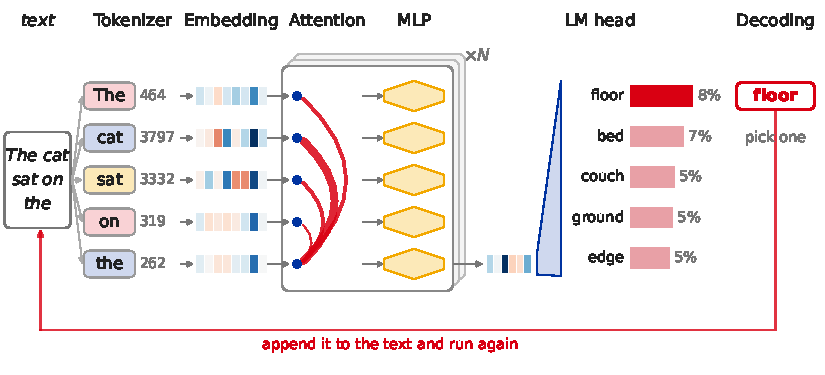
\includegraphics[width=\linewidth]{roadmap_pretraining_pass.pdf}\end{center}
  \vskip -2pt
  {\small The forward pass is built (LLM-1 to LLM-6). Today: where its 124M numbers come from.}
\end{frame}

\begin{frame}{Where we are: the life of a model}
  \begin{center}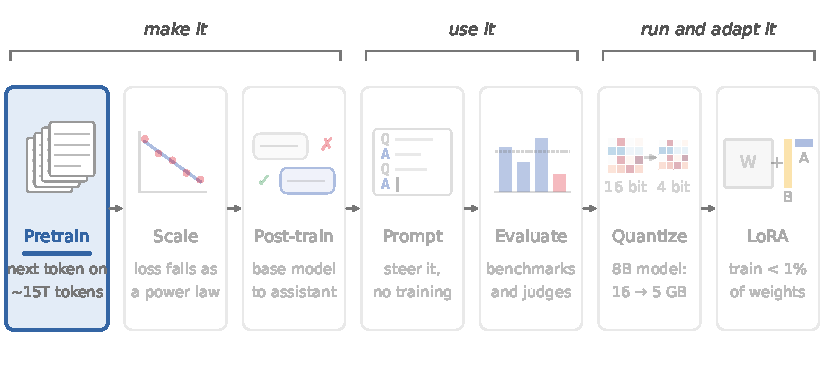
\includegraphics[width=\linewidth]{roadmap_pretraining_life.pdf}\end{center}
  \vskip -2pt
  {\small Today: the first box. Everything after it starts from what it produces, a
  \textbf{base model}.}
\end{frame}

% ============================================================ COLD OPEN (py_src/pretraining_figs.py --gpt2)
\begin{frame}{Finish these}
  \vskip 4pt
  Two famous openings. GPT-2 small gets each one and writes the next 48 tokens, always taking the
  most likely one (greedy, LLM-6).

  \vskip 10pt
  \begin{columns}[T]
    \column{0.48\textwidth}
      \keybox{\textbf{A.} ``Permission is hereby granted, free of charge, to any person obtaining
      a copy \ldots''\\[3pt]{\scriptsize\color{gray} the MIT software licence}}
    \column{0.48\textwidth}
      \keybox{\textbf{B.} ``Four score and seven years ago our fathers brought forth
      \ldots''\\[3pt]{\scriptsize\color{gray} the Gettysburg Address, 1863}}
  \end{columns}

  \vskip 14pt
  \trapbox{\textbf{Predict first:} which one does it continue word for word? Both, one, or
  neither?}
\end{frame}

\begin{frame}{The licence, not the speech}
  \begin{center}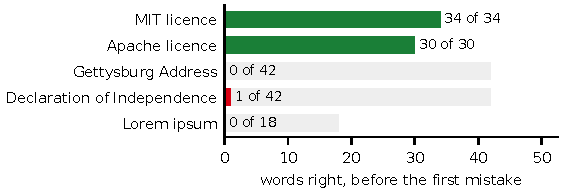
\includegraphics[width=0.68\linewidth]{pre_recite.pdf}\end{center}
  \vskip -4pt
  {\small \textbf{A}: all 34 words right, and the Apache licence 30 of 30. \textbf{B}: wrong from
  the first word (``the first of the great and great, \ldots''); the Declaration of Independence
  fares no better. Lorem ipsum (0) is common on the web, but dataset filters often drop it (C4
  removes every page that contains it).}

  \vskip 4pt
  \keybox{Famous is not the same as frequent. A software licence is pasted into countless source
  files; a speech is quoted far less often. Today: where the 124M numbers come from, and why they
  memorised the licence and not the speech.}
  \vskip 1pt
  \src{Cached GPT-2 small, greedy, 48 new tokens; words compared after collapsing whitespace.}
\end{frame}

\begin{frame}{Outline}
  \tableofcontents
\end{frame}

% ============================================================ 1. THE OBJECTIVE
\section{The objective}
\sectiontransition{The objective}{Hide part of the text, and make the model guess it.}

\begin{frame}{You have seen one already}
  \vskip 6pt
  \begin{itemize}
    \item LLM-4: with the causal mask, one forward pass makes a guess at \textbf{every} position:
      the next token, from everything before it.
    \item Each guess is scored by $-\ln p(\text{the right token})$; the \textbf{loss} is the
      average over all the guesses.
    \item Gradient descent (ch11) nudges all 124M numbers so the right tokens become a little
      more likely. Repeat on the next batch, billions of times.
  \end{itemize}

  \vskip 8pt
  That is the whole objective. Most of today is about the text it runs on.

  \vskip 8pt
  \keybox{But is ``guess the next token'' the only way to turn raw text into a training signal?}
\end{frame}

\begin{frame}{Five ways to hide text}
  \begin{center}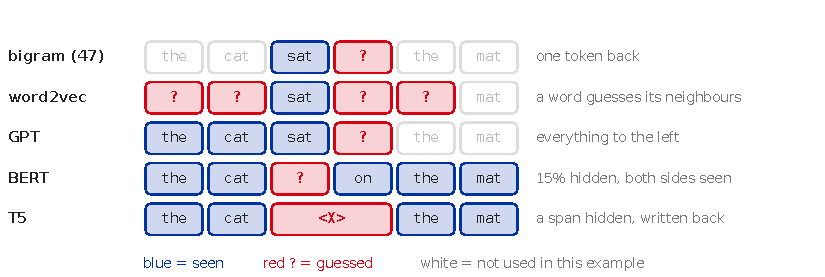
\includegraphics[width=\linewidth]{pre_objectives.pdf}\end{center}
  \vskip -2pt
  {\small Each row is one training example on the same sentence. The model learns whatever it
  needs to fill the red cells. Next: word2vec, BERT and T5 (GPT's row is LLM-4's).}
\end{frame}

\begin{frame}{word2vec: a word and its neighbours}
  \begin{center}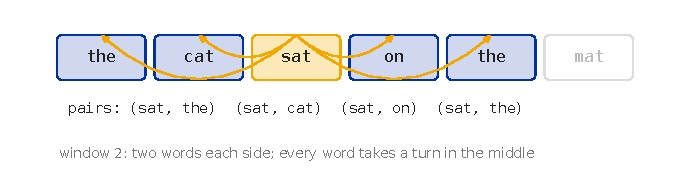
\includegraphics[width=0.84\linewidth]{pre_w2v_pairs.pdf}\end{center}
  \vskip -2pt
  \small
  \begin{itemize}
    \item \textbf{Skip-gram} (Mikolov et al., 2013): every word guesses each neighbour in a window.
      ``sat'' gives 4 pairs; the whole six-word sentence gives 18.
    \item No word order inside the window, nothing beyond it, no network around it: just a table
      with one row of numbers per word - the kind of table LLM-2 showed.
  \end{itemize}
\end{frame}

\begin{frame}{Why word2vec learns meaning}
  \vskip 4pt
  Each word gets a vector. For a pair seen in the text, say (sat, cat):
  \begin{itemize}
    \item push the dot product $u_{\text{sat}} \cdot v_{\text{cat}}$ \textbf{up};
    \item pick a few random words (``negative samples'', say 5) and push their dot products with
      $u_{\text{sat}}$ \textbf{down}.
  \end{itemize}
  \vskip 2pt
  \begin{center}
    $\text{loss} = -\ln \sigma(u_{\text{sat}} \cdot v_{\text{cat}})
    - \sum_{k=1}^{5} \ln \sigma(-u_{\text{sat}} \cdot v_{k})$
  \end{center}
  \vskip 2pt
  {\small ($\sigma$ is the sigmoid, and $-\ln \sigma(x)$ shrinks as $x$ grows: minimising the first
  term raises $u_{\text{sat}} \cdot v_{\text{cat}}$, the second lowers the random ones. Each word
  keeps two vectors, $u$ as the centre and $v$ as a neighbour; the $u$'s are the table you keep.)}

  \vskip 6pt
  \keybox{``cat'' and ``dog'' both sit next to ``the'', ``fed'' and ``sat'', so they are pushed
  towards the same places: meaning from the company a word keeps. Cheap and fast, but with no
  order and no depth it cannot write a sentence.}
\end{frame}

\begin{frame}{BERT: hide 15\%, see both sides}
  \vskip 4pt
  \begin{itemize}
    \item Pick \textbf{15\%} of the tokens (Devlin et al., 2018). Of those: 80\% become
      \texttt{[MASK]}, 10\% become a random token, 10\% stay as they are. Predict the original
      at all of them.
    \item Why not always \texttt{[MASK]}? When the model is used, there is no \texttt{[MASK]} in
      the input; the 10\% + 10\% stop it from relying on one.
    \item Every other token is visible, \textbf{on both sides}: LLM-5's mask A.
  \end{itemize}

  \vskip 8pt
  \trapbox{So BERT cannot write left to right (LLM-5's cold open). What it is good at is the
  vectors: a sentence read in both directions. Embedding models for search descend from it
  (the RAG chapter).}

  \vskip 4pt
  {\small And only the 15\% are scored, so each sentence gives fewer training signals.}
\end{frame}

\begin{frame}{T5: hide whole spans}
  \vskip 6pt
  The T5 paper's own example (Raffel et al., 2020):

  \vskip 8pt
  \begin{center}
  \begin{tabular}{rl}
    original & \texttt{Thank you for inviting me to your party last week.} \\[4pt]
    input & \texttt{Thank you \textcolor{armred}{<X>} me to your party \textcolor{armred}{<Y>}
      week.} \\[4pt]
    target & \texttt{\textcolor{armred}{<X>} for inviting \textcolor{armred}{<Y>} last
      \textcolor{armred}{<Z>}}
  \end{tabular}
  \end{center}

  \vskip 10pt
  \begin{itemize}
    \item 15\% of the tokens are dropped, in spans of 3 on average; each span becomes one
      \textbf{sentinel} token, and a final sentinel (\texttt{<Z>}) marks the end of the target.
    \item The encoder reads the input; the decoder writes the missing spans back (LLM-5's mask C).
  \end{itemize}
\end{frame}

\begin{frame}{Why next-token won}
  \vskip 8pt
  \begin{itemize}
    \item \textbf{Every position is a target.} A 1,024-token window gives 1,023 guesses (LLM-4);
      on the same 1,024 tokens, BERT's 15\% gives about 154.
    \item \textbf{It writes.} The model you pretrain is already the one that generates.
    \item \textbf{Any text will do.} No labels and no masking recipe: the next token is always
      sitting right there.
  \end{itemize}

  \vskip 12pt
  \takebox{Not a cleverer objective: more signal per sentence, and a model that writes. LLM-5
  said the same about the architecture.}
\end{frame}

% ============================================================ 2. ONE TRAINING STEP
\section{One training step, by hand}
\sectiontransition{One training step}{From three documents to one number.}

\begin{frame}{Pack the documents}
  \begin{center}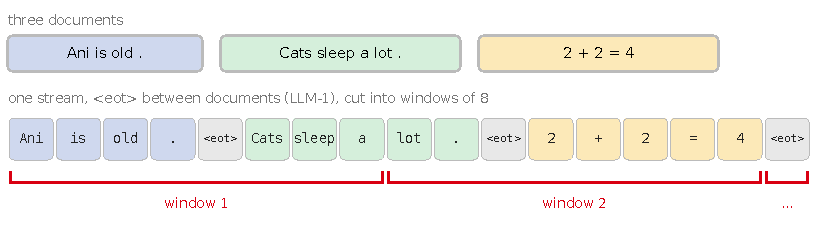
\includegraphics[width=\linewidth]{pre_packing.pdf}\end{center}
  \vskip -4pt
  \small
  \begin{itemize}
    \item Documents have every length; the GPU wants equal windows. So join them with the
      end-of-text token between (GPT-2's \texttt{<|endoftext|>}, LLM-1) and cut every 8 tokens
      (GPT-2: every 1,024). Toy tokens here: one word each.
    \item Both windows cross a document boundary. The \texttt{<eot>} tells the model that what
      follows is unrelated.
  \end{itemize}
\end{frame}

\begin{frame}{One window, seven guesses}
  \begin{center}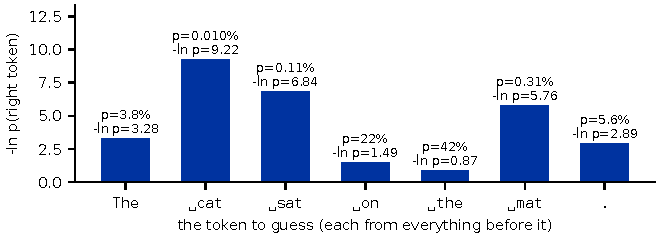
\includegraphics[width=0.80\linewidth]{pre_window_loss.pdf}\end{center}
  \vskip -4pt
  {\small Real GPT-2 on \texttt{<eot>The cat sat on the mat.}: 8 tokens, 7 guesses (the first token
  has nothing before it), all in one pass (LLM-4). ($\textvisiblespace$ = the leading space.)}

  \vskip 4pt
  {\small\textbf{By hand:} $\text{loss} = (3.28 + 9.22 + 6.84 + 1.49 + 0.87 + 5.76 + 2.89) / 7
  = 30.35 / 7 = \mathbf{4.34}$}

  \vskip 4pt
  \keybox{`` cat'' at 0.010\% is the big surprise: 30\% of the whole loss. Training pushes every
  right token up, and the biggest surprises carry the most loss.}
\end{frame}

\begin{frame}{Loss to perplexity}
  \vskip 6pt
  The name inventor (47) turned loss into something you can feel:
  \vskip 4pt
  \begin{center}
    $\text{perplexity} = e^{\text{loss}} = e^{4.34} \approx \mathbf{77}$
  \end{center}

  \vskip 6pt
  \begin{itemize}
    \item As unsure as if it picked among 77 equally likely tokens at every step. Guessing
      uniformly over GPT-2's vocabulary would be 50,257; a perfect model, 1.
    \item Seven guesses are a noisy estimate. Papers average over millions of tokens of held-out
      text.
  \end{itemize}

  \vskip 8pt
  \watchbox{Perplexity counts surprise \emph{per token}. That is fine for one model on one text.
  It goes wrong as soon as the tokens are not the same size.}
\end{frame}

\begin{frame}{Perplexity across tokenizers lies}
  \vskip 2pt
  {\small Toy numbers. One Armenian sentence of 45 characters (83 bytes: each letter is 2). Two
  tokenizers: byte-level pieces, 80 tokens and 70 bits of surprise in total; Armenian-aware, 12
  tokens and 60 bits. (Bits are nats $/ \ln 2$; $2^{\text{bits}} = e^{\text{nats}}$, the same
  perplexity.)}
  \begin{center}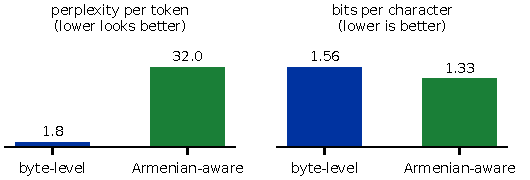
\includegraphics[width=0.64\linewidth]{pre_bpc.pdf}\end{center}
  \vskip -4pt
  {\small Per token: $70/80 = 0.875$ bits, perplexity $2^{0.875} = 1.8$; against $60/12 = 5$ bits,
  $2^5 = 32$. The byte-level model looks 17$\times$ better. Per character: $70/45 = 1.56$ against
  $60/45 = 1.33$ bits. It is worse.}

  \vskip 4pt
  \keybox{Short tokens are easy to guess one at a time (LLM-1's token tax). Compare \textbf{bits
  per character} (or per byte) on the same text, never per-token perplexity across tokenizers or
  languages.}
\end{frame}

% ============================================================ 3. THE DATA
\section{The data}
\sectiontransition{The data}{Most of the work is throwing text away.}

\begin{frame}{How much text}
  \vskip 6pt
  \begin{center}
  \small
  \begin{tabular}{lp{0.70\linewidth}}
    \toprule
    \textbf{GPT-2} (2019) & WebText: pages linked from Reddit posts with at least 3 karma (net
      upvotes);
      about 8 million documents, 40 GB. Wikipedia removed (it overlaps with test sets). \\[3pt]
    \textbf{FineWeb} (2024, open) & 15T tokens of English, from 96 snapshots of Common Crawl, a
      non-profit that crawls the web and gives the pages away. \\[3pt]
    \textbf{Llama 3} (2024) & trained on about 15.6T tokens; the Llama 3 paper puts Llama 2 at
      1.8T. \\
    \bottomrule
  \end{tabular}
  \end{center}

  \vskip 8pt
  \keybox{In five years, from 40 GB of hand-picked links to trillions of tokens of filtered web.
  At that scale nobody reads the data. Rules and classifiers decide what a model sees.}
\end{frame}

\begin{frame}{The funnel}
  \begin{center}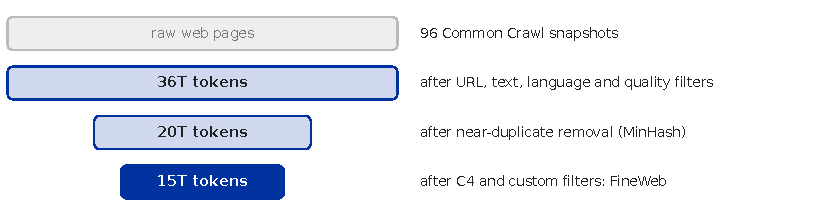
\includegraphics[width=\linewidth]{pre_funnel.pdf}\end{center}
  \vskip -4pt
  \small
  \begin{itemize}
    \item The first filters, in order: block bad URLs; pull the main text out of the HTML; keep
      English (a classifier's confidence $\geq 0.65$); drop low-quality and repetitive pages.
    \item Then remove near-duplicates (in three frames), apply most of C4's rules and FineWeb's
      own, and mask email and IP addresses.
    \item From 36T to 15T: more than half of what survived the first filters is thrown away.
  \end{itemize}
  \src{Penedo et al. (2024), ``The FineWeb Datasets'', arXiv 2406.17557.}
\end{frame}

\begin{frame}{Clean this page by hand}
  \begin{columns}[c]
    \column{0.58\textwidth}
      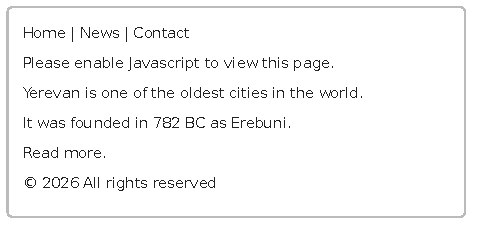
\includegraphics[width=\linewidth]{pre_c4_page_q.pdf}
    \column{0.40\textwidth}
      {\small Four of C4's rules (the T5 paper, 2019):
      \begin{enumerate}
        \item a line must end in . ! ? or a closing quote;
        \item a line needs at least 5 words;
        \item a line that mentions Javascript goes;
        \item a page needs at least 3 sentences.
      \end{enumerate}}
  \end{columns}

  \vskip 10pt
  \trapbox{\textbf{Predict first:} what is left of this page?}
\end{frame}

\begin{frame}{Two good sentences, and the page still goes}
  \begin{center}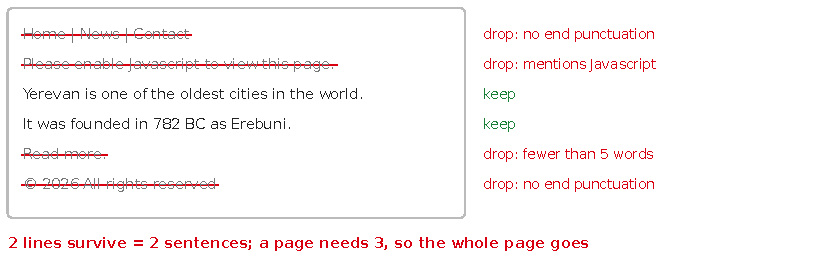
\includegraphics[width=\linewidth]{pre_c4_page.pdf}\end{center}
  \vskip -2pt
  {\small Four lines fail a line rule. The two that pass are real content, but two sentences are
  fewer than three, so rule 4 removes the page.}

  \vskip 4pt
  \watchbox{Rules like these are blunt. In FineWeb's tests the end-punctuation rule helped most
  on its own, but removed about 30\% of all tokens, so FineWeb dropped it. Every rule trades the
  junk it removes against the good text it loses.}
\end{frame}

\begin{frame}{Duplicates}
  \vskip 2pt
  \begin{itemize}
    \item The web repeats itself: mirrors, templates, boilerplate, licences. FineWeb compares
      documents by their sets of 5-word sequences (MinHash) and keeps one of each group that is
      at least 75\% alike.
    \item Lee et al. (2022) found one 61-word sentence repeated over \textbf{60,000} times in C4.
      Trained on deduplicated data, models emitted memorised text \textbf{10$\times$} less often.
    \item Carlini et al. (2022): memorisation grows log-linearly with the number of copies, with
      model size, and with the length of the prompt.
  \end{itemize}

  \vskip 8pt
  \keybox{That is the cold open. The licence is the extreme duplicate; the speech is quoted in a
  few places. The model holds what it saw many times.}
\end{frame}

\begin{frame}{How much of the web is Armenian?}
  \begin{center}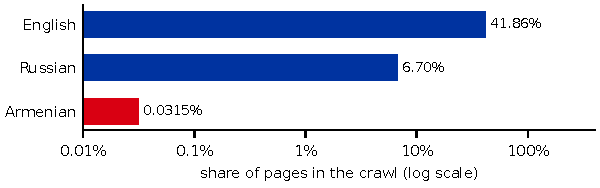
\includegraphics[width=0.74\linewidth]{pre_languages.pdf}\end{center}
  \vskip -4pt
  {\small Common Crawl's latest crawl (CC-MAIN-2026-39), share of pages by main language: about
  \textbf{1,330 English pages for every Armenian one}. FineWeb-2, the multilingual sibling: 634
  million Armenian words (1.76M documents) against 589 billion Russian words.}

  \vskip 4pt
  \keybox{A model sees Armenian about as often as the web writes it. Few examples, plus LLM-1's
  token tax, are a large part of why answers in Armenian are weaker. And a language classifier
  decides what counts as Armenian in the first place.}
\end{frame}

\begin{frame}{The mixture}
  \begin{columns}[c]
    \column{0.58\textwidth}
      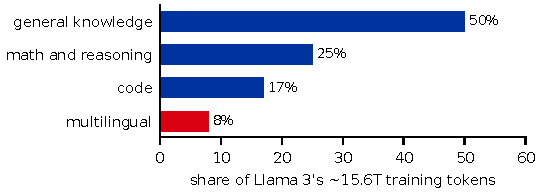
\includegraphics[width=\linewidth]{pre_mixture.pdf}
    \column{0.40\textwidth}
      {\small A lab does not train on the funnel's output as it is. It decides how much of each
      kind of text goes in, and can give scarce, valuable kinds (code, maths) more weight than
      their share of the web.

      \vskip 6pt
      Llama 3's mix, over about 15.6T tokens.}
  \end{columns}

  \vskip 10pt
  \takebox{Every language except English shares the red 8\%. The mixture is a decision, and it
  shapes what the model is good at as much as the architecture does.}
\end{frame}

% ============================================================ 4. WHAT COMES OUT
\section{What comes out}
\sectiontransition{What comes out}{A base model: it continues documents.}

\begin{frame}{Watching it learn}
  \vskip 4pt
  Karpathy reproducing GPT-2 small (2025): 1 million tokens per step, 32,000 steps, about 33
  billion tokens in all. Every 20 steps the model writes a sample.
  \vskip 6pt
  \begin{itemize}
    \item \textbf{Step 20:} completely random text. The network is still random.
    \item \textbf{About 1\% in (step 420):} ``since she is mine it's a part of the information
      should discuss my father great companions Gordon showed me sitting over at''. Word pairs
      make sense; the sentence does not.
    \item \textbf{After the whole run} (the rest takes a day or two): fairly coherent English.
  \end{itemize}

  \vskip 8pt
  \keybox{The loss falls smoothly; what the samples show is local structure first (which word
  follows which), then longer-range sense.}
  \vskip 2pt
  \src{Karpathy, ``Deep Dive into LLMs like ChatGPT'' (2025), 35:00-38:00.}
\end{frame}

\begin{frame}{It recites, and it leaks}
  \vskip 4pt
  \begin{itemize}
    \item \textbf{It recites what it saw many times}: the licences in the cold open.
    \item \textbf{You have seen this before.} The name inventor (47, section 12), trained
      8$\times$ too long (1,200 epochs): the share of its ``inventions'' that were real training
      names climbed from 0\% to 32\%.
    \item \textbf{It can leak what it saw once.} Carlini et al. (2021) pulled hundreds of
      verbatim sequences out of GPT-2, including names, phone numbers and email addresses, each
      from a single training document.
  \end{itemize}

  \vskip 10pt
  \trapbox{Training data is not read and forgotten. That is why FineWeb masks email addresses, and
  why removing duplicates matters for privacy as well as quality.}
\end{frame}

\begin{frame}{It continues documents}
  \begin{center}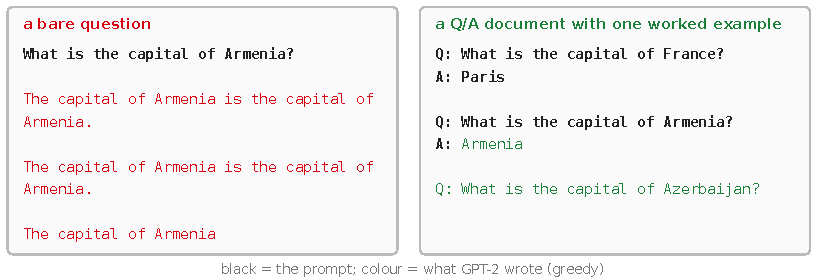
\includegraphics[width=0.86\linewidth]{pre_base_model.pdf}\end{center}
  \vskip -4pt
  {\small Left: no answer, just more text about the question (here, a loop). Right: as a Q/A
  document the format works - a short answer, then the next question, because Q/A pages have
  many. The answer is wrong: 124M parameters do not hold ``Yerevan''.}

  \vskip 4pt
  \takebox{A base model is a \textbf{document simulator}. To get an answer, the answer has to be
  the likely continuation. LLM-9 trains that behaviour in.}
\end{frame}

\begin{frame}{GPT-1, GPT-2, GPT-3}
  \vskip 6pt
  \begin{center}
  \small
  \begin{tabular}{llp{0.62\linewidth}}
    \toprule
    \textbf{Model} & \textbf{Size} & \textbf{How it was used for a task} \\
    \midrule
    GPT-1 (2018) & 117M & pretrain, then fine-tune a copy for each task \\[2pt]
    GPT-2 (2019) & 1.5B & no fine-tuning: write the task into the text (``TL;DR:'' after an
      article makes it summarise). The largest of four sizes; today's runs used the smallest,
      124M \\[2pt]
    GPT-3 (2020) & 175B & a few worked examples in the prompt: \textbf{few-shot}, no weight
      updates \\
    \bottomrule
  \end{tabular}
  \end{center}

  \vskip 10pt
  \keybox{The same objective all three times. What changed was scale, and how much of the task
  could move from training into the prompt. How the few-shot gain grows with size is LLM-8;
  how to write such prompts is LLM-10.}
\end{frame}

% ============================================================ CLOSE
\begin{frame}{Recap}
  \small
  \begin{itemize}
    \item \textbf{The objective}: hide text and guess it. Next-token won: every position is a
      target, and it writes. word2vec, BERT and T5 hide text in other ways.
    \item \textbf{One step}: pack documents with \texttt{<eot>}, cut windows, average
      $-\ln p$ of the right tokens. Perplexity $= e^{\text{loss}}$; across tokenizers compare
      bits per character, not per token.
    \item \textbf{The data}: most of the work is filtering (FineWeb: 36T $\to$ 20T $\to$ 15T
      tokens) and removing duplicates. Armenian is 0.03\% of the pages; the mixture is a
      decision.
    \item \textbf{What comes out}: a base model, a document simulator. It recites what it saw
      often, can leak what it saw once, and continues instead of answering.
  \end{itemize}
\end{frame}

\begin{frame}{Next on the map}
  \begin{center}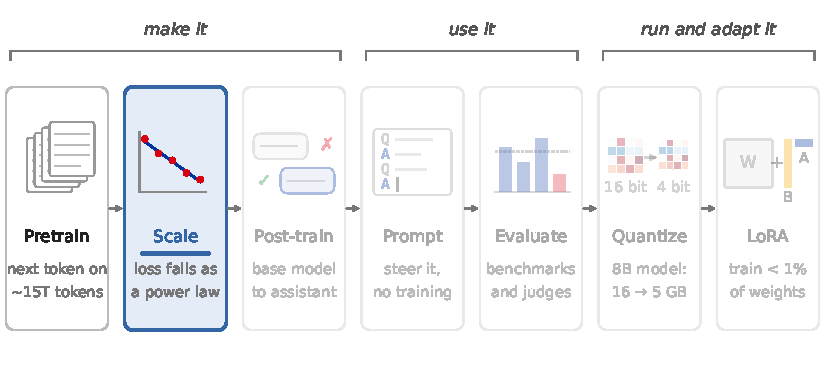
\includegraphics[width=\linewidth]{roadmap_scaling_life.pdf}\end{center}
  \vskip -2pt
  {\small Next (LLM-8): how big a model, and how much data, for a given compute budget.}
\end{frame}

\begin{frame}{Sources \& further reading}
  \footnotesize
  \begin{itemize}
    \item Mikolov et al. (2013), ``Distributed Representations of Words and Phrases and their
      Compositionality'' (skip-gram, negative sampling).
    \item Devlin et al. (2018), ``BERT''; Raffel et al. (2020), ``Exploring the Limits of
      Transfer Learning with a Unified Text-to-Text Transformer'' (T5, C4, span corruption).
    \item Radford et al. (2018, 2019), GPT-1 and GPT-2 (WebText); Brown et al. (2020), GPT-3.
    \item Penedo et al. (2024), ``The FineWeb Datasets'', arXiv 2406.17557; FineWeb-2 dataset
      card (Hugging Face); Common Crawl language statistics, CC-MAIN-2026-39.
    \item Lee et al. (2022), ``Deduplicating Training Data Makes Language Models Better'';
      Carlini et al. (2021), ``Extracting Training Data from Large Language Models''; Carlini et
      al. (2022), ``Quantifying Memorization Across Neural Language Models''.
    \item Llama Team (2024), ``The Llama 3 Herd of Models''; Karpathy (2025), ``Deep Dive into
      LLMs like ChatGPT''.
  \end{itemize}
  \vskip 2pt
  \src{Figures: \texttt{py\_src/pretraining\_figs.py}. Real: GPT-2's recitations, its loss on one
  window, its two answers (cached model, one run), and the published numbers above. Toy: the
  objectives, packing, word2vec pairs, the tokenizer comparison, the web page.}
\end{frame}

\end{document}

% ============================================================================
% Provenance:
%   Deck: LLM-7 Pretraining (14_llms), session 7 of the LLM chapter. Built 2026-10-06 from
%   LLM7_pretraining_OUTLINE.md, which follows the critique in LLM_CHAPTER_PLAN.md (LLM-7) and the
%   recommended answers in INTERVIEW_QUEUE.md (instructor: "do all queue items"; DECISIONS #76).
%   Spine: data-led (objective family -> one step by hand -> data -> what comes out). Cold open:
%   one greedy run of the cached GPT-2 on five openings (MIT 34/34 words, Apache 30/30,
%   Gettysburg 0/42, Declaration 1/42, lorem ipsum 0/18). All four real pieces used.
%   Sources ported: dl4nlp 07 (CLM / MLM, BERT's 80/10/10), 01 (word2vec), the name-inventor
%   practical (47: perplexity, section 12's copying curve), Karpathy's transcript (35:00-38:00),
%   sources/llm_training/07_llama3 (15.6T, the mix). Facts checked 2026-10-06: the outline's
%   "Facts checked" table (FineWeb, C4 rules and the T5 example from the paper's text, BERT, the
%   Common Crawl and FineWeb-2 numbers, Carlini 2021/2022, Lee 2022, GPT-2's WebText).
%   Numbers: every printed number is asserted in py_src/pretraining_figs.py (recitation counts,
%   the window's seven -ln p and their printed sum 30.35 / mean 4.34 / e^4.34 = 77 - the unrounded
%   value is 76.5 -, the toy bits-per-character numbers, the C4 verdicts, 1,330 English pages per
%   Armenian page).
%   Cut (plan's list): ELMo, NSP/SOP, contrastive learning, compute tables (-> LLM-8), n-gram
%   smoothing, synthetic data. Not here: "autocomplete is not a chatbot" with the password
%   (LLM-9's cold open) - the Q/A run is a different prompt.
%   STUDENT REVIEW 2026-10-06 (one Sonnet agent, rendered PNGs only; ~87k tokens, 104 s). It
%   re-did the sums (30.35 / 7, e^4.34, the 18 pairs, 154, 1,330) and found them right. Caught a
%   real error: the toy "byte-level, 40 tokens for 45 Armenian characters" is impossible (2 bytes
%   per letter) - now 80 tokens (83 bytes), so per-token perplexity 2^0.875 = 1.8 vs 32, "17x"
%   (checked). Also applied: bits vs nats said once; GPT-2's 1.5B is the largest of four sizes;
%   "most of C4's rules" (FineWeb dropped end punctuation); the lorem ipsum and Declaration bars
%   explained; n tokens -> n - 1 guesses; why -ln sigma pushes the dot product up; the final <Z>;
%   both windows cross a boundary; karma; the classifier's confidence; no unsupported
%   "repeats"; the Q/A panel named as a worked example; larger panel and verdict text.
% ============================================================================
